%
%    Autor: Simon Walker
%			simon.walker@hsr.ch
%
%	 Dieses LaTeX Dokument benutzt eine Karteikartenklasse welche von Ronny Bergmann <mail@rbergmann.info> entwickelt wurde version 1.8b
%	 Die Dokumentation und die Karteikartenklasse sind unter folgendem Link erhältlich
%    https://github.com/kellertuer/Kartei

%------------------------------------------------------------
% Lernkarten zum Fach ELT2,
%------------------------------------------------------------

%Nach fertiger Entwicklung grid auf none setzen
\documentclass[a7paper,10pt,grid=rear% %Grösse der Karteikarten auswählen (A5-A9)
%,toc			%Komentarlöschen falls eine Zusammenstellung gewünscht wird
,print			%Komentar löschen falls eine Ausdruckversion erstellt werden soll
]{kartei}

%Erzeugt im Antwortfeld eine Minipage um zu verhindern dass über den seitlichen Rad geschrieben wird
%Achtung dadurch wird die überprüfung von zu grossen Antworten unterdrückt
\newenvironment{lk}[1]{\begin{karte}{#1}\begin{minipage}{0.9\textwidth}}{\end{minipage}\end{karte}}

%\newcommand*{\lk}[2]{\begin{karte}{#1}
%		\begin{minipage}{\textwidth}
%			#2
%		\end{minipage}
%	}

\usepackage[utf8]{inputenc} %UTF8
\usepackage{hyperref}

\usepackage{amsmath}
\usepackage{bm}
\usepackage{paralist}

\begin{document}
	\setcardpagelayout
	
	\fach{ELT2}
	\kommentar{Elektrostatik} %Thema

%--------------------------------------------------------
%Lektion 4
%--------------------------------------------------------

\begin{lk}{Was sind elektrische Leiter?}
	Medium mit frei beweglichen Ladungsträger
\end{lk}	

\begin{lk}{Was ist eine Äquipotentialfläche?}
	Fläche auf der überall das gleiche elektrostatische Potential ist.
\end{lk}	

\begin{lk}{Warum kennt Elektrostatik keinen Widerstand?}
	Wir haben keine Strömung. $ -> $ Es wird keine Ladung bewegt.
\end{lk}

\begin{lk}{Was ist Influenz?}
	Die Beeinflussung eines Leiters durch das elektrostatische Feld.\\
	Das elektrische Feld führt zu einer Ausrichtung der Ladungsträger im Innern des Leiters. Dadurch entsteht ein Gegenfeld welches wiederum das Elektrische Feld beeinflusst. Das effektive elektrische Feld ist die Überlagerung des Homogenen Feldes und dem Gegenfeld des Leiters.
	\center{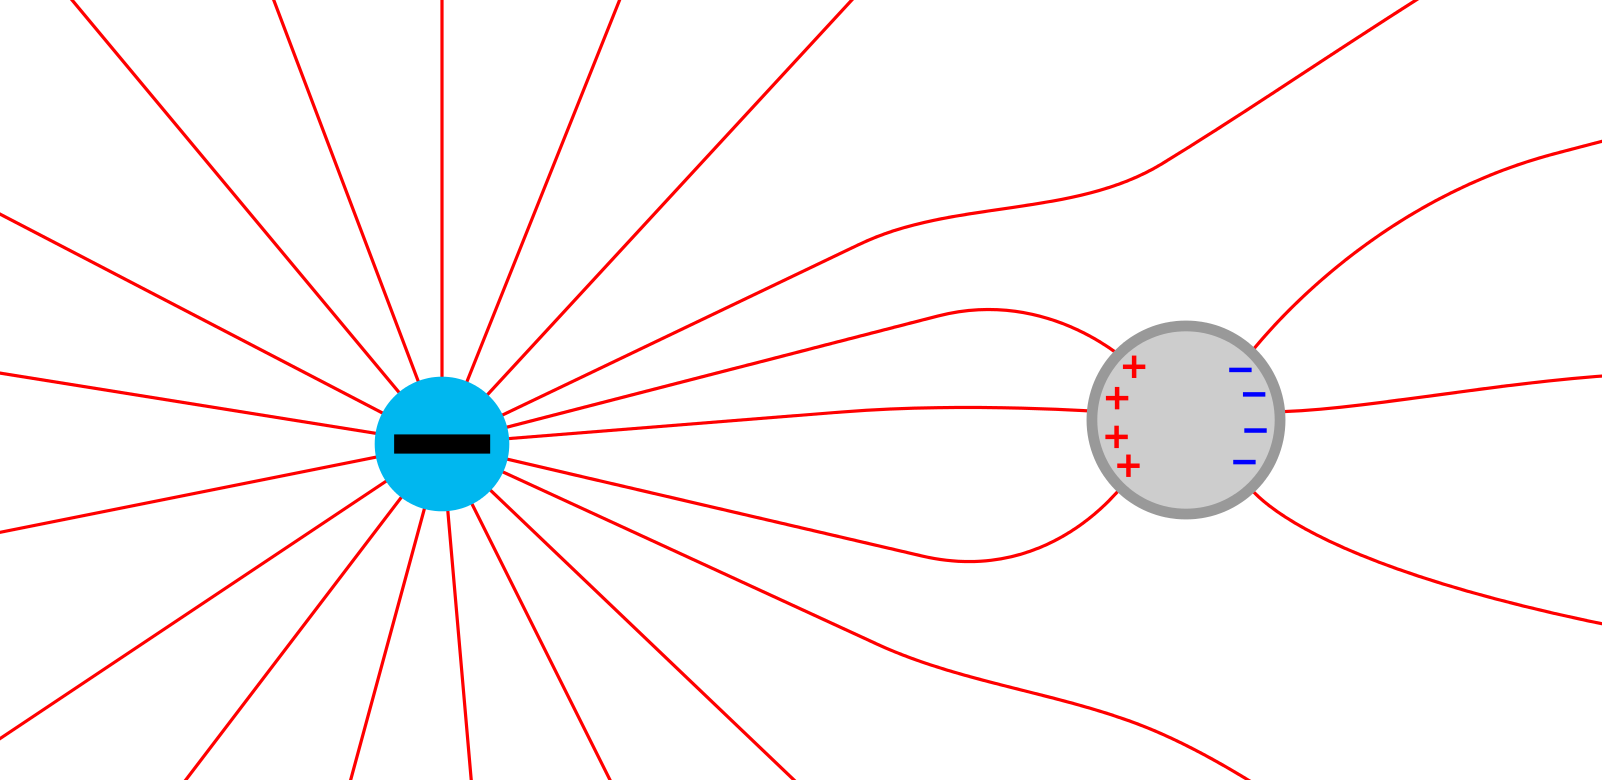
\includegraphics[width=0.55\textwidth]{pics/ES_Influenz.png}} %Von Stündle - Eigenes Werk, CC0, https://commons.wikimedia.org/w/index.php?curid=18191603
\end{lk}

\begin{lk}{Wie funktioniert ein Faradayscher Käfig?}
	Im Innern eines Leiters gibt es einen Feldfreien Raum da sich die Ladungen durch die Influenz ausrichten und dadurch ein Gegenfeld erzeugen. Dieses Gegenfeld hebt im Innern des Leiters das Elektrische Feld auf.
	
	\center{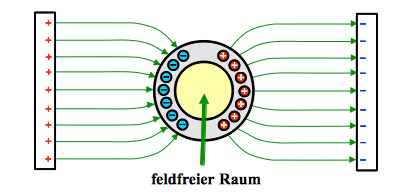
\includegraphics[width=0.7\textwidth]{pics/ES_FaradayscherKaefig.png}} %http://elektronik-kurs.net/elektrotechnik/einfluss-des-elektrischen-feldes-auf-materialien/
\end{lk}

\begin{lk}{Was besagt das Gauss-Gesetz des elektrostatischen Felds?}
	Gesamter Fluss durch eine Oberfläche entspricht der darin enthalten Ladung.
\end{lk}

\begin{lk}{Wie gross ist die Oberfläche einer Kugel mit Radius r?}
	\center{\huge{$ 4 \cdot \pi \cdot r^2 $}}
\end{lk}

%--------------------------------------------------------
%Lektion 5
%--------------------------------------------------------

\begin{lk}{Was ist eine Spiegelladung?}
	\begin{minipage}{0.7\textwidth}
		Eine Spiegelladung ist eine Virtuelle Ladung welche die gleich gross ist wie die original Ladung einfach mit negativem Vorzeichen. Dadurch kann der originaler Teil dargestellt werden und berechnet werden. Der Gespiegelte Teil existiert allerdings nicht und desshalb ist dort das Feld nicht so berechenbar\\
		\textbf{Wichtig: Ein Spiegel spigelt immer alles!}
	\end{minipage}
	\begin{minipage}{0.29\textwidth}
			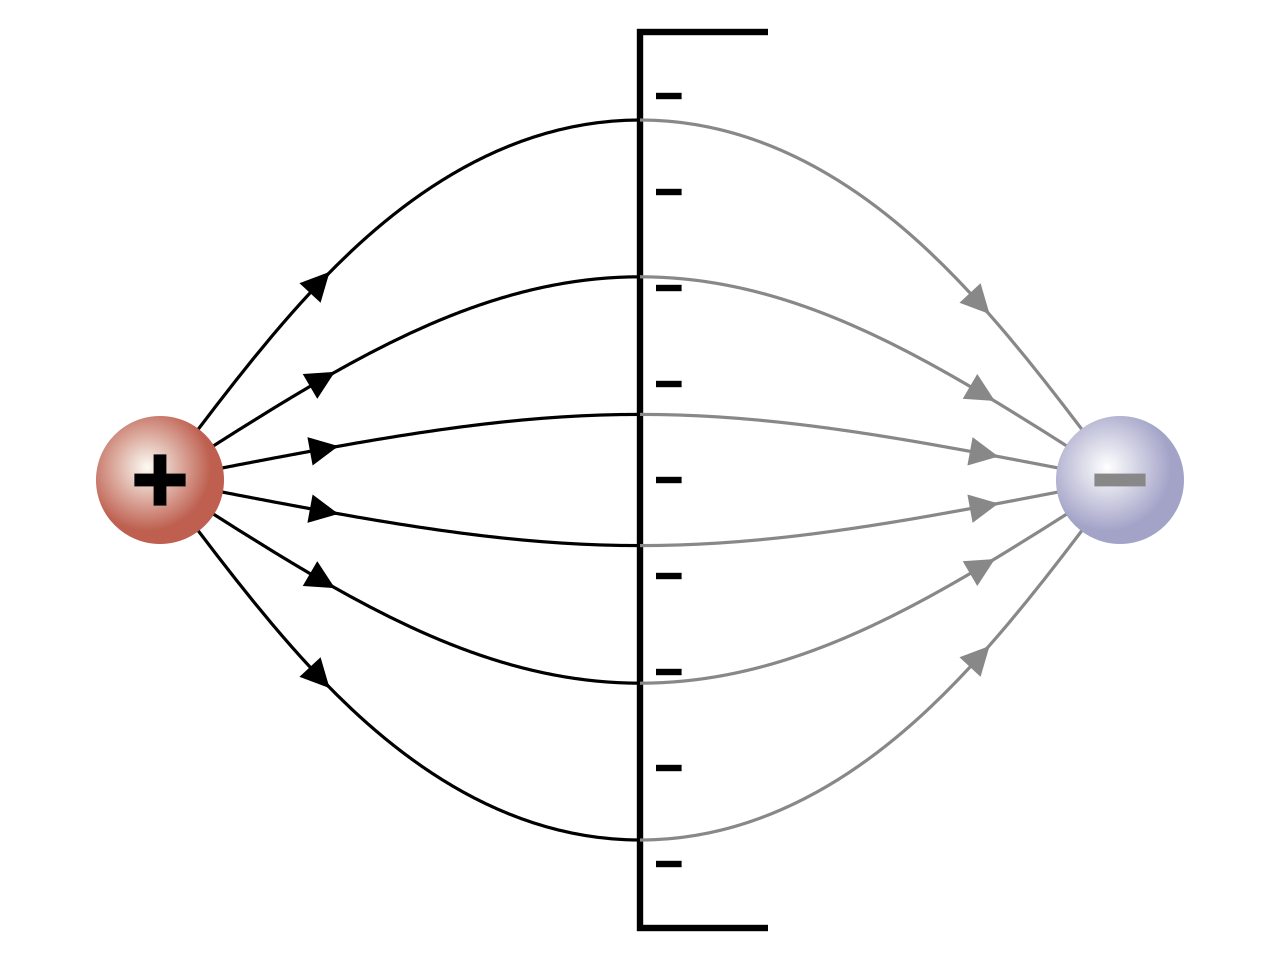
\includegraphics[width=\textwidth]{pics/ES_Spiegelladung.png} %By Paeng 12:53, 30. Nov. 2008 (CET) - selbst erstellt nach PNG-Vorlage von Benutzer:Degreen: :Bild:Spiegelladung.jpg, GFDL, https://commons.wikimedia.org/w/index.php?curid=60070873
	\end{minipage}
\end{lk}

\begin{lk}{Wodurch zeichnet sich ein (elektrischer) Nichtleiter aus?}
	Ein Nichtleiter hat keine Freien Ladungsträger.\\
	Alle Ladungsträger sind gebunden.
\end{lk}

\begin{lk}{Was sind gebundene Ladungen?}
	\begin{itemize}
		\item Die Ladungen sind nicht Frei bewegbar.
		\item Die Ladungsträger lassen sich ausrichten.
	\end{itemize}
\end{lk}

\begin{lk}{Worum handelt es sich bei der Polarisation und welche Arten davon gibt es?}
	\begin{compactitem}
		\item Ausrichtung der Ladung am Elektrischen Feld (Es gibt dadurch ein Dipol) Es wird ein Elektrisches Feld im Inneren des Materials geben, welches gegen das äussere Feld wirkt.
		\item Es gibt 3 Arten:
		\begin{compactitem}
			\item Verschiebungspolarisation (schnell, schwach)
			\item Orientierungspolarisation (Moleküle bei Dipolen)
			\item Ionenpolarisation
		\end{compactitem}
	\end{compactitem} 
	\begin{center}
		\begin{minipage}{0.18\textwidth}
			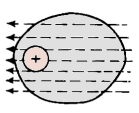
\includegraphics[width=\textwidth]{pics/ES_Ausrichtungspolarisation.png}\\
		\end{minipage}
		\begin{minipage}{0.18\textwidth}
			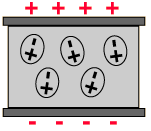
\includegraphics[width=\textwidth]{pics/ES_Orientierungspolarisation.png}\\ % http://hydrogen.physik.uni-wuppertal.de/hyperphysics/hyperphysics/hbase/electric/dielec.html Grafik Modifiziert
		\end{minipage}
		\begin{minipage}{0.18\textwidth}
			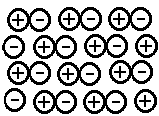
\includegraphics[width=\textwidth]{pics/ES_Ionenpolarisation.png}\\ %Eigene Grafik
		\end{minipage}
	\end{center}
\end{lk}

\begin{lk}{Wie nennt man die Auswirkung eines elektrischen Felds auf einen Leiter und auf einen Nichtleiter?}
	\begin{itemize}
		\item Leiter: Influenz
		\item Nichtleiter: Polarisation
	\end{itemize}
\end{lk}	

\begin{lk}{Wie lauten die Grenzbedingungen des elektrischen Felds?} %Zeichnung in Arbeit
	\begin{itemize}
		\item Die Normalen der elektrischen Flüssen bleiben gleich
		\item Die Tangentialen der elektrischen Felder bleiben gleich
	\end{itemize}
\end{lk}	

%--------------------------------------------------------
%Lektion 6
%--------------------------------------------------------

\begin{lk}{Was bedeutet Permittivität?}
	Die Permittivität ($ \varepsilon $), auch dielektrische Leitfähigkeit genannt, zeig an wie gut sich ein Isolator Polarisieren lässt\\
	Je höher die Permittivität desto schlechter ist die Durchlässigkeit für Elektrische Felder
\end{lk}	

\begin{lk}{Welche beiden Arten des Gaussschen Gesetzes gibt es?}
	Fluss durch die Geschlossene Oberfläche eines Körpers ist gleich der darin enthaltenen Ladung.\\[12pt]
	Da es zwei verschiedene arten von Ladungen gibt (gebunden und nicht gebunden), gibt es auch 2 Verschiedene Gesetze. Diese finden Anwendung bei der Betrachtung von Grenzübergängen.
\end{lk}

\begin{lk}{Was bezeichnet man als elektrische Kapazität C?}
	Fähigkeit Ladung zu speichern. Oder anderst gesagt: Wie viel Ladung kann gespeichert werden bei gewissen Spannungen.
	
	Kapazität lat für Fassungsvermögen
	
	\huge{$ Q = C \cdot U \quad \rightarrow \quad C = \dfrac{Q}{U}$}
\end{lk}	

\begin{lk}{Was ist der Typische Wertebereich von elektrischen Kapazitäten}
	Von Pico Farad bis zu Milli Farad.
\end{lk}	

\begin{lk}{Wie lautet $[C] = F$ in SI Einheiten?} 
	\center{
	$ \dfrac{1}{2}\cdot C \cdot U^2 = \dfrac{1}{2} \cdot \dfrac{Q^2}{C} $\\[12pt]
	$ [C] = F = \dfrac{[Q^2]}{[W]} = \dfrac{A^2 \cdot s^4}{kg \cdot m^2} $
	}
\end{lk}	

\begin{lk}{Was ist die Formel für Plattenkondensatoren}
	\center{\huge{$ C = \dfrac{\varepsilon \cdot A}{d} $}}\\[12pt]
	\center{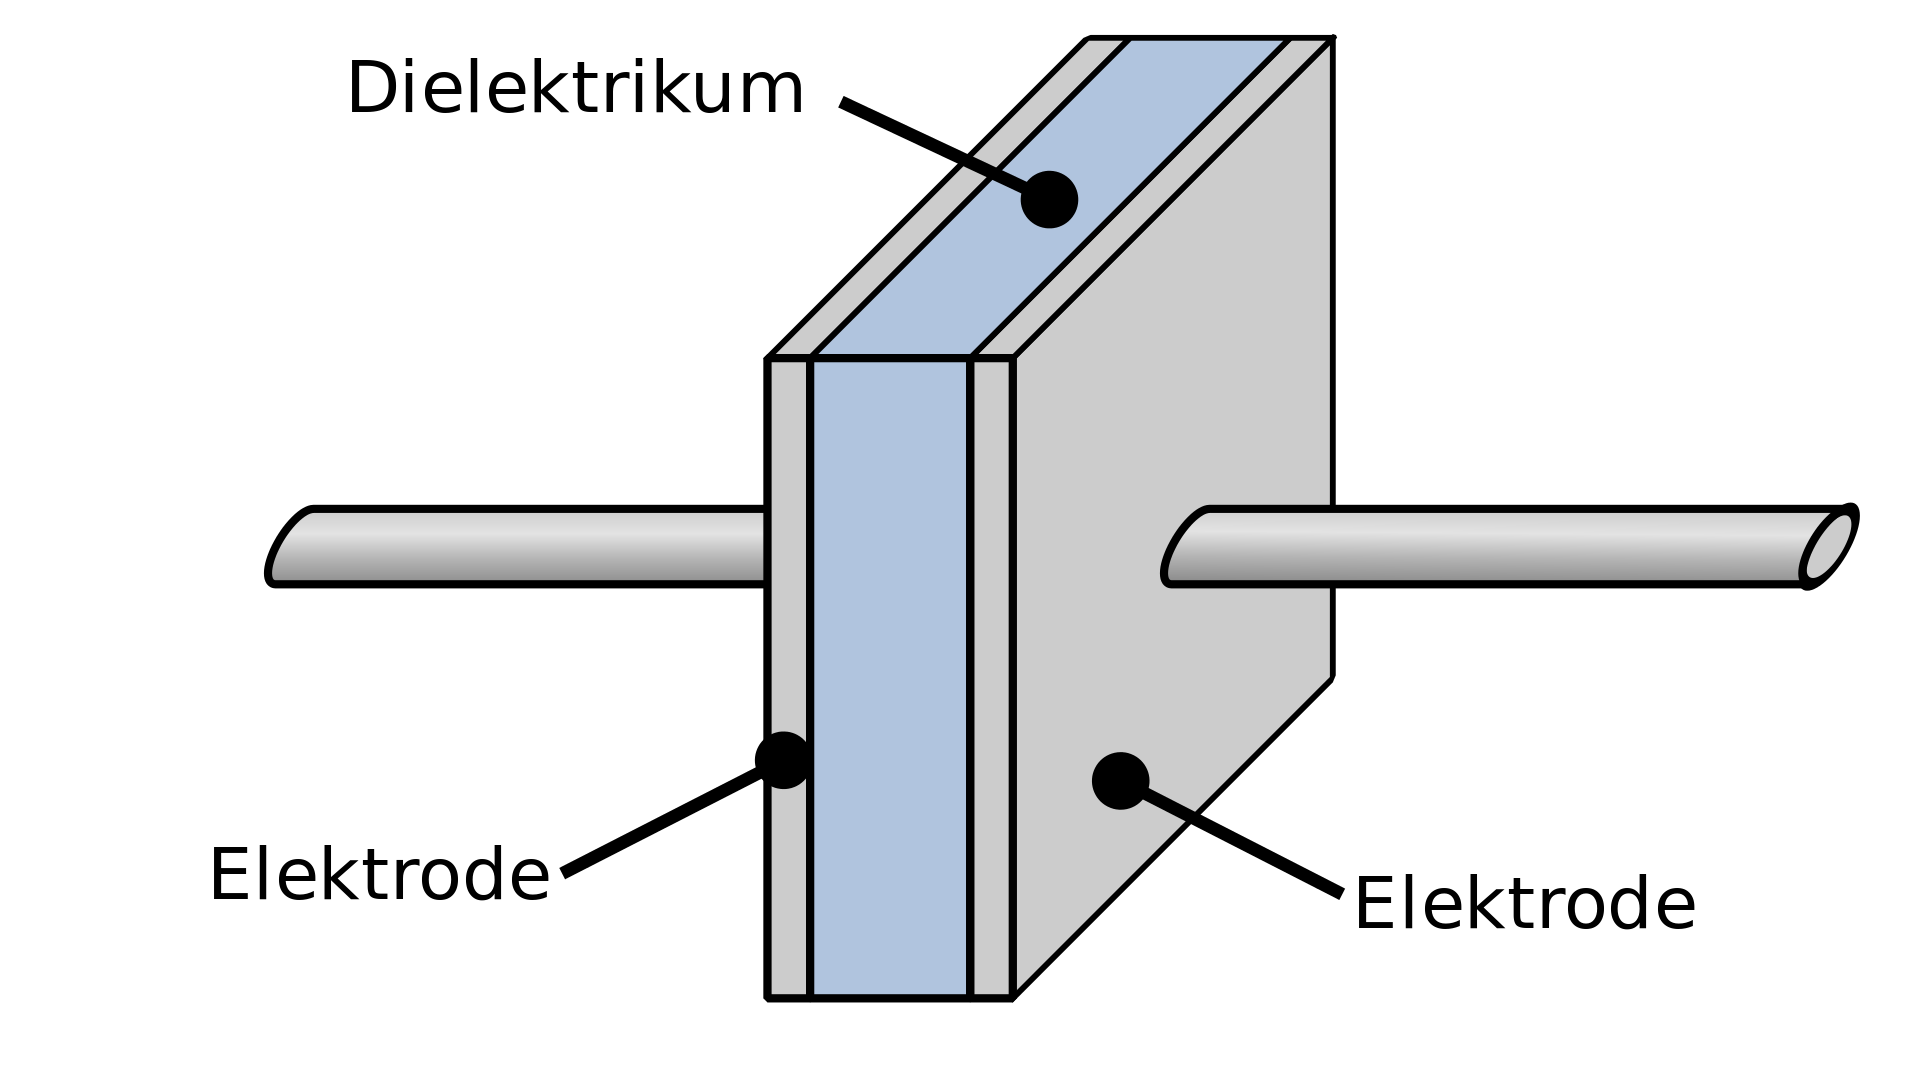
\includegraphics[width=0.5\textwidth]{pics/ES_Plattenkondensator.png}} %Von Cepheiden - Eigenes Werk, CC BY-SA 3.0, https://commons.wikimedia.org/w/index.php?curid=5613903
\end{lk}	


%--------------------------------------------------------
%Lektion 7
%--------------------------------------------------------

\begin{lk}{Was ist der Unterschied zwischen elektrischem Fluss und elektrischer Strömung?}
	\begin{compactitem}
		\item Beides sind kontinuierliche Grössen.
		\item Elektrischer Fluss (Statisch), kein Ladungstransport.
		\item Elektrische Strömung (Dynamik), Ladungstransport.
	\end{compactitem}
\end{lk}

\begin{lk}{Was ist Strom?}
	\textbf{Ladungstransport}
\end{lk}

\begin{lk}{Wie lautet [R] in SI-Grundeinheiten?}
	$ \dfrac{[U]}{[I]} = \dfrac{[P \cdot t]}{[I \cdot t][I]} = \dfrac{Kg \cdot \frac{m^2}{s^2}}{A \cdot s \cdot A} = $\\[12pt]
	\LARGE{ $ \dfrac{Kg \cdot m^2}{A^2 \cdot s^3} $ }
\end{lk}

%--------------------------------------------------------
%Testat
%--------------------------------------------------------
\begin{lk}{Was ist die Coulomb-Kraft und wie wird sie berechnet?}
	Die Coulomb-Kraft beschreibt die Kraft zwischen zwei Punkt-Ladungen in Abhängigkeit von dessen Abstand zueinander.\\[12pt]
	\LARGE{ $ \bm{F} = \dfrac{Q_1 \cdot Q_2}{4 \cdot \pi \cdot \varepsilon_0 \cdot R^2} \cdot \bm{\hat{R}} $} \\[12pt]
	\normalsize Wobei $ \bm{\hat{R}} $ immer der von der Ursache zur Wirkung zeigt.
\end{lk}

\begin{lk}{Wie berechnet man die Elektrische Feldstärke an einem bestimmten Punkt von einer oder mehreren Punktladungen?}
	\LARGE{ $ \vec{E} = \dfrac{Q}{4 \cdot \pi \cdot \varepsilon_0 \cdot r^2} \cdot \hat{r} $} \\[12pt]
	\normalsize  Bei mehreren Ladungen werd<en die einzelnen Felder überlagert.
\end{lk}
		
\end{document}